\subsection{Planning second half}
% 1 page
To get the project back on track we need to apply careful planning. We need an overview of the remaining parts of the project, an estimate of how much time we have left, and a carefully structured plan on the order of the activities we have left to do.\\
We have divided the planning into four parts.

We start out by looking at the development methods that we want to use. We give a brief introduction to the method, and explain how we applied it to help the project back on track.

After this we describe the estimation methods we use. The estimation methods should help us make accurate estimations and based on these, decision. This, in turn, helps us to meet the deadline, as most of our estimations should be correct or close to.

When we have found how much time we need, we need to find out how much time we have available. For this we use a couple of methods for planning the time. Those methods are explained, and our usage is analyzed.

As the last, but possibly the most important part, we look into how our project recovery has affected the quality. Less time to do roughly the same work must have some effect on the quality, since the time, cost, and quality of a product are constrained by each other (see figure \ref{fig:timeCostsQuality})\cite[p. 191]{PM}. In the final part we will analyze this aspect of our project.

\begin{figure}[t]
  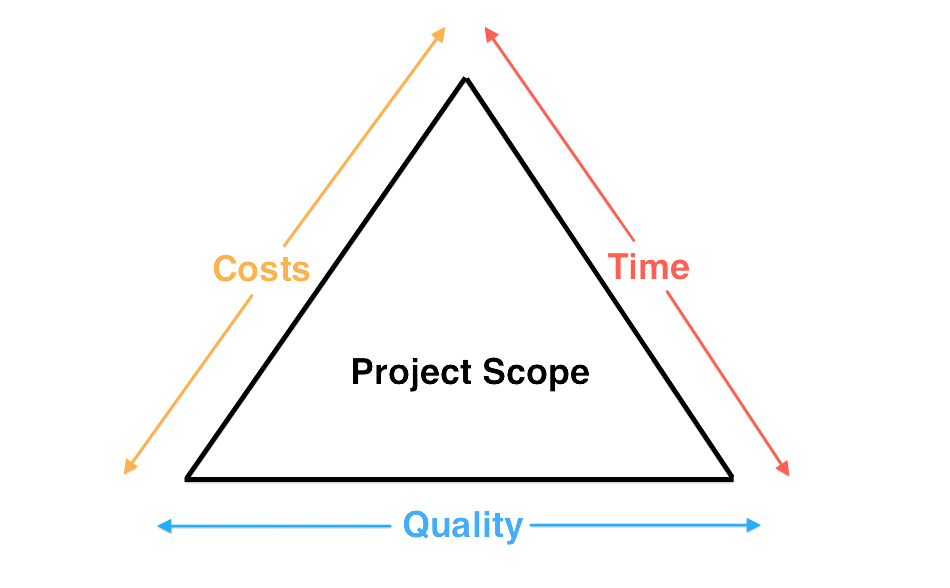
\includegraphics[width=\textwidth]{illustrations/timeCostsQuality}
  \caption{The triple constraint: When the requirements to costs, timescale, or quality change, the resources assigned to the other aspects must change accordingly as well.}
  \label{fig:timeCostsQuality}
\end{figure}